\documentclass{article}
\usepackage[utf8]{inputenc}
\usepackage{caption}
\usepackage{amsmath}
\usepackage{amssymb}
\usepackage{mathtools}
\usepackage{multicol}
\usepackage{graphicx}
\usepackage{wrapfig}
\usepackage{float}
\usepackage[makeroom]{cancel}

\graphicspath{ {./images/} }

\renewcommand{\baselinestretch}{1.5} % line spacing
\newcommand{\fline}{\par\noindent\rule{\textwidth}{0.1pt}} % horizontal line (wide)

\title{Dynamics Lab\\Acceleration with a Pulley}
\author{Peter Zhang}

\begin{document}

\maketitle
\newpage
\tableofcontents
\newpage


\section{Purpose}
To compare the experimental acceleration to the theoretical acceleration for an object moving horizontally while being pulled by a hanging mass.

\section{Data Tables}

\begin{center}
	\begin{tabular}{|c|c|}
		\hline
		Variable & Measured Value\\
		\hline \hline
		$m_{car}$ & $545.7g\pm1g$\\
		\hline
		$m_{weight\ 1}$ & $20g\pm0.2g$\\
		\hline
		$m_{weight\ 2}$ & $50g\pm0.2g$\\
		\hline
		$m_{t}$ & $m_{weight\ 1} + m_{weight\ 2} = 70g\pm0.4g$\\
		\hline
	\end{tabular}
	\captionof{table}{Experimental Values}
\end{center}

\begin{figure}[H]
	\centering
	\fbox{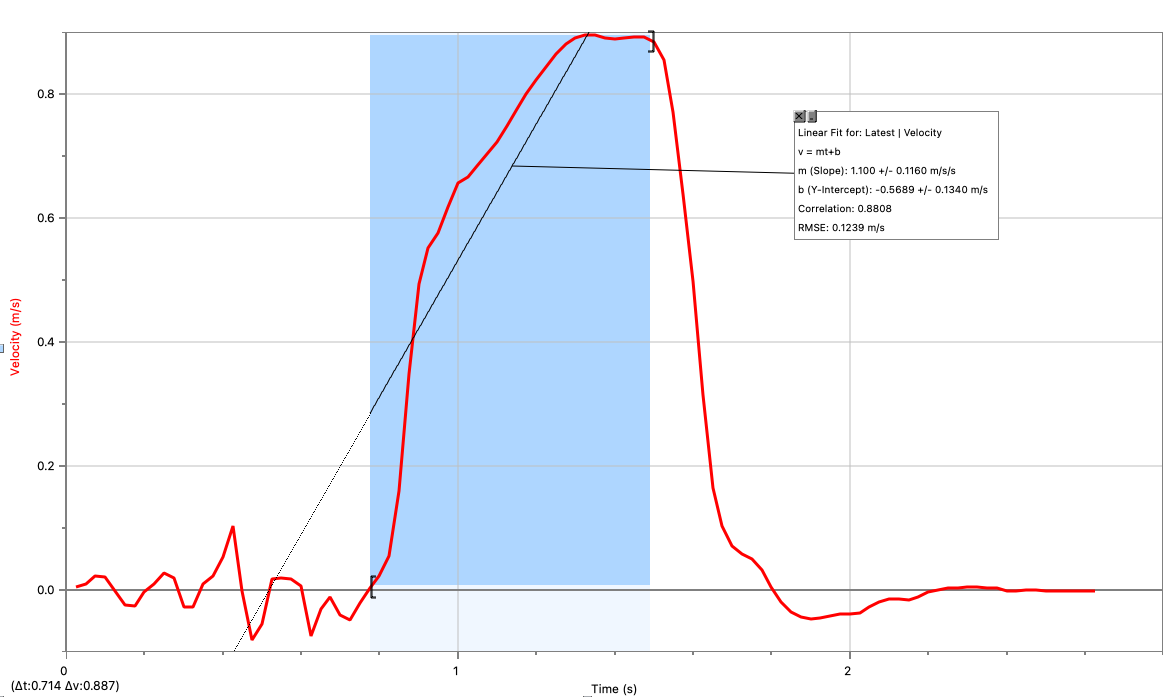
\includegraphics[width=\textwidth]{images/graph_line_x.png}}
	\captionof{figure}{Velocity Time Graph with Line of Best Fit}
\end{figure}

\begin{figure}[H]
	\centering
	\fbox{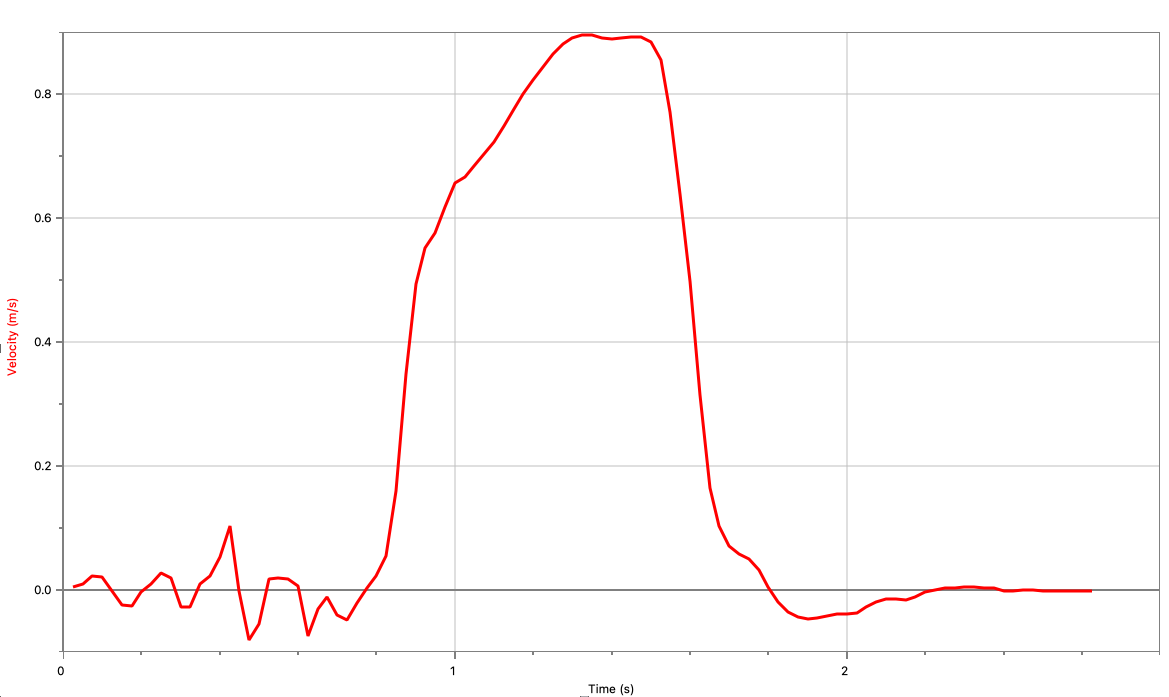
\includegraphics[width=\textwidth]{images/graph_no_line.png}}
	\captionof{figure}{Velocity Time Graph without Line of Best Fit}
\end{figure}

\begin{figure}[H]
	\centering
	\fbox{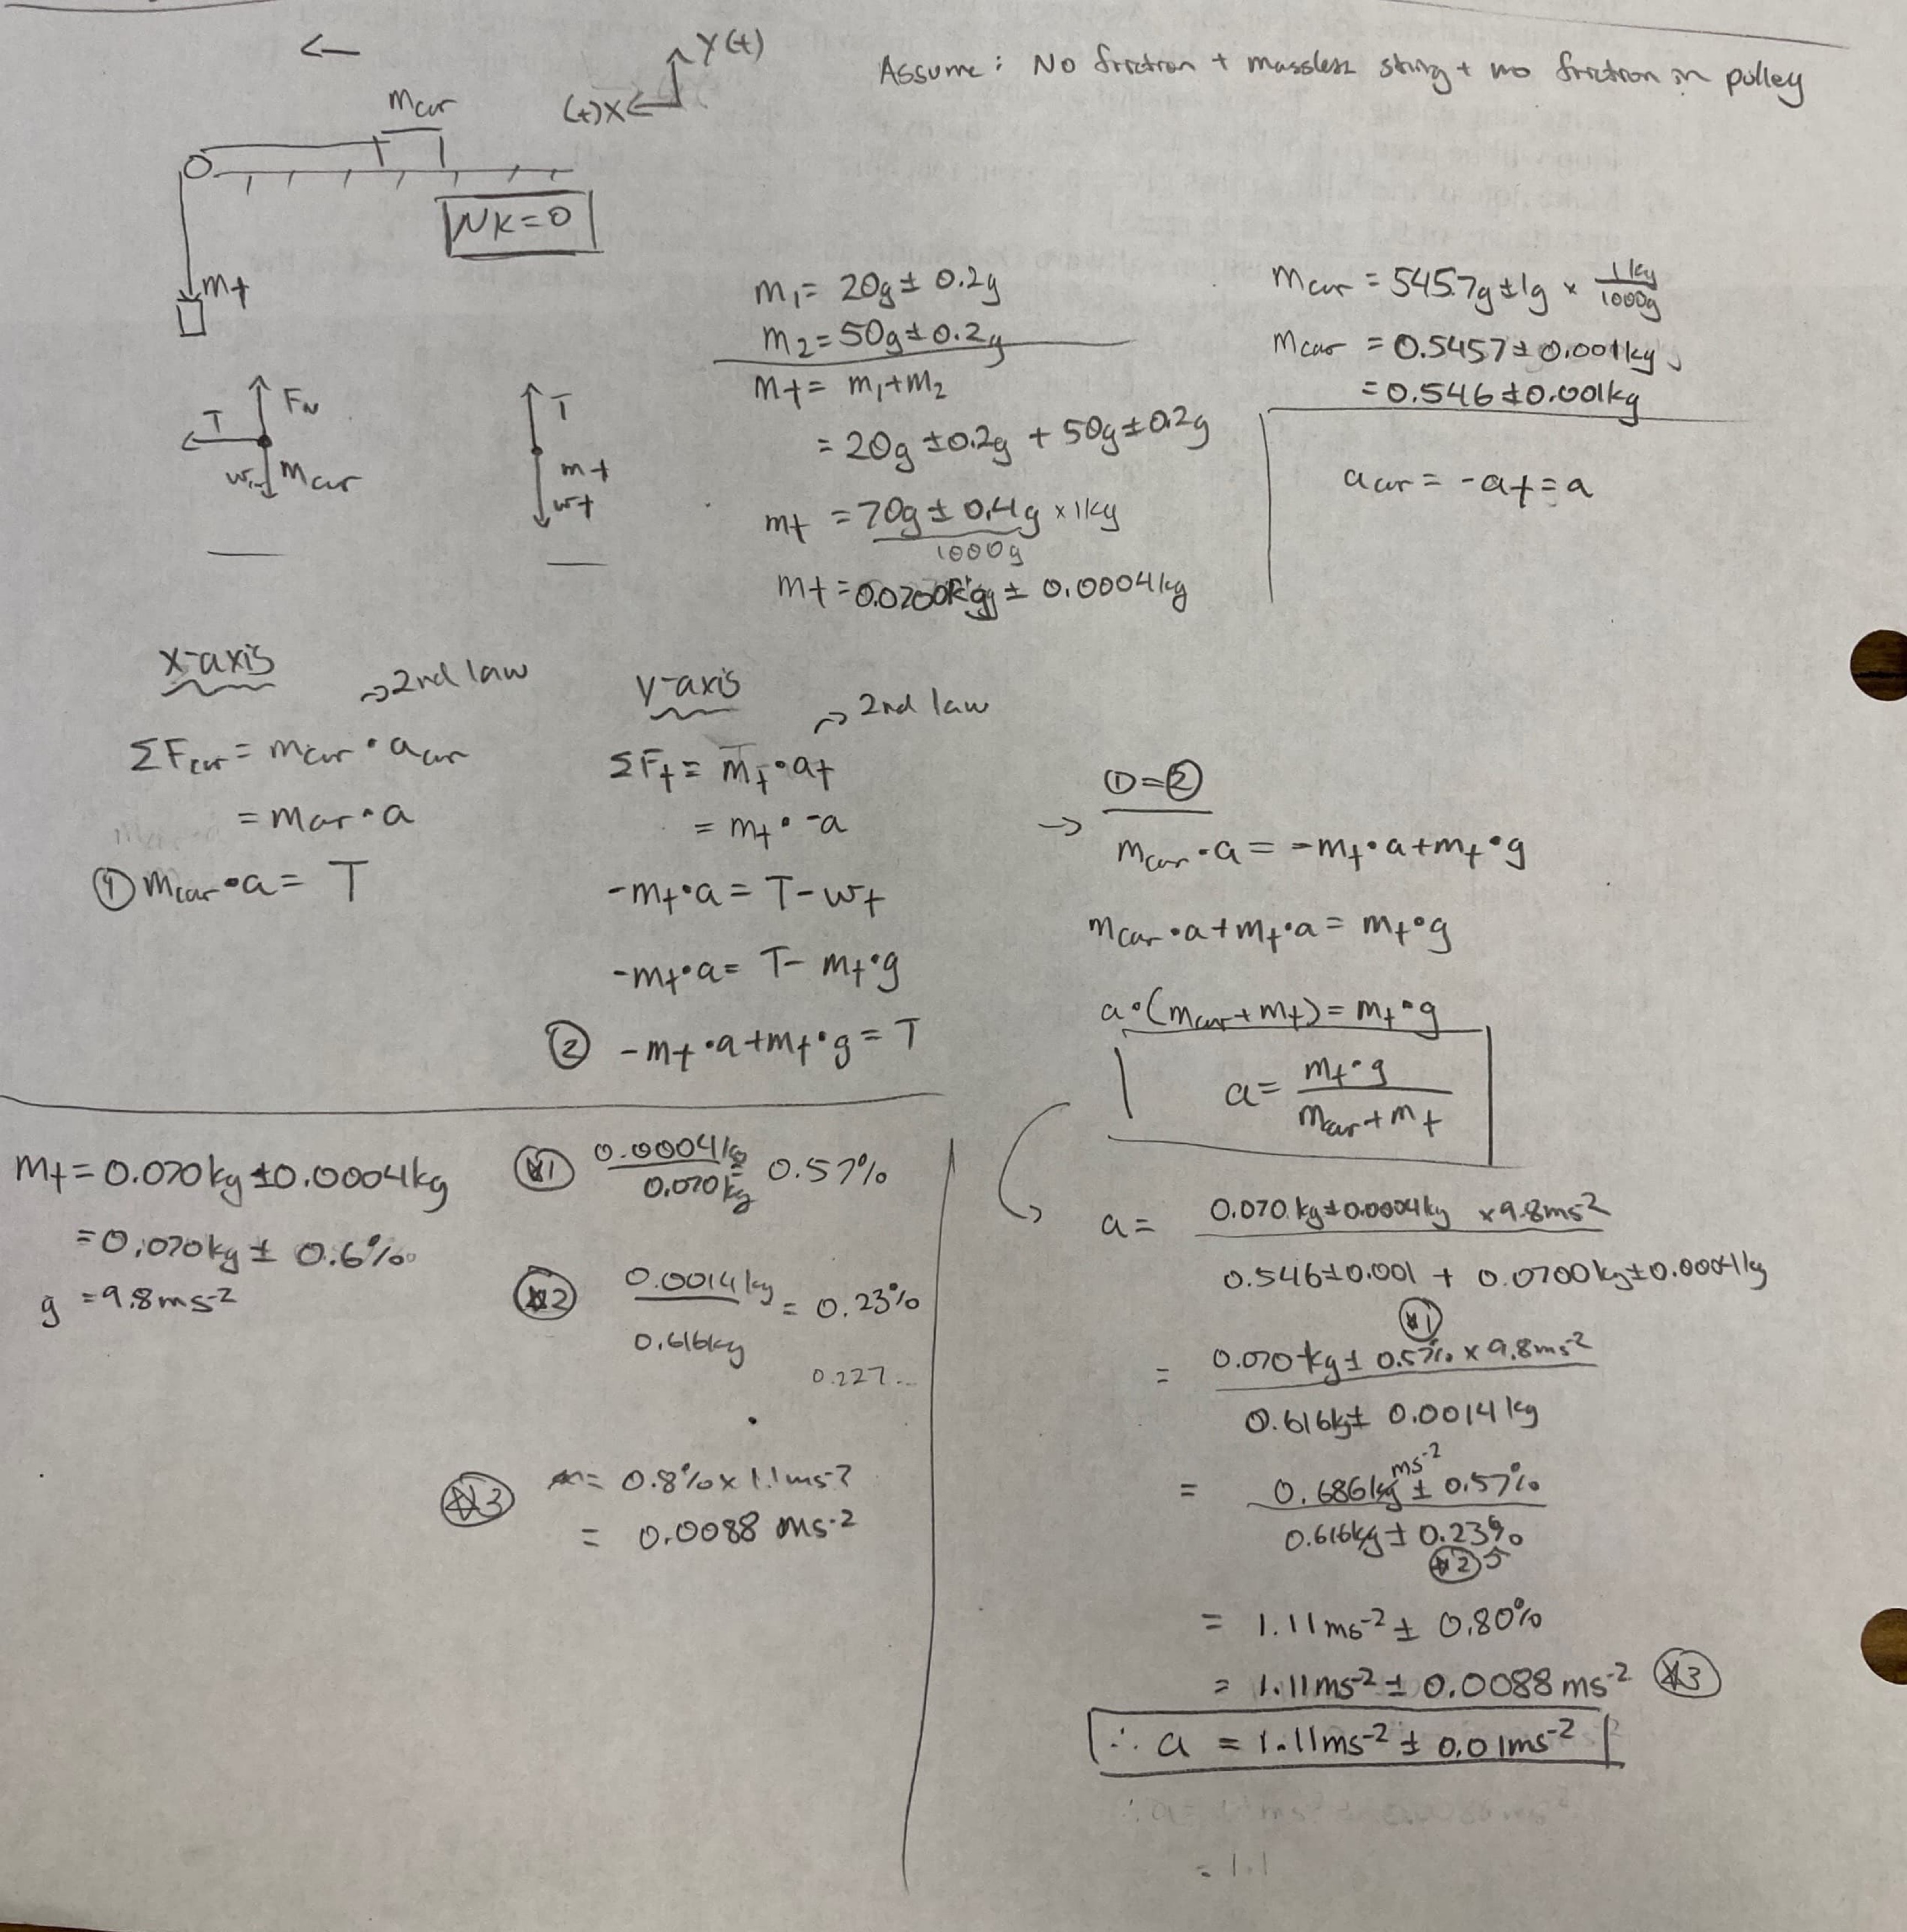
\includegraphics[width=\textwidth]{images/calculations.JPG}}
	\captionof{figure}{Calculations}
\end{figure}

\section{Analysis}

\section{Discussion}






\end{document}
